\documentstyle[epsfig,12pt]{article}

\topmargin -.8cm
\oddsidemargin  10.5pt
\evensidemargin  10.5pt
\textheight  612pt
\textwidth  432pt

\newcommand{\be}{\begin{equation}}
\newcommand{\ee}{\end{equation}}
\newcommand{\ba}{\begin{eqnarray}}
\newcommand{\ea}{\end{eqnarray}}
\newcommand{\bd}{\begin{displaymath}}
\newcommand{\ed}{\end{displaymath}}

\def\thalf{{\textstyle{\frac{1}{2}}}}
\def\tthalf{{\textstyle{\frac{3}{2}}}}
\def\oneth{{\textstyle{\frac{1}{3}}}}
\def\twoth{{\textstyle{\frac{2}{3}}}}
\def\oneqt{{\textstyle{\frac{1}{4}}}}
\def\ttqt{{\textstyle{\frac{3}{4}}}}
\def\fth{{\textstyle{\frac{4}{3}}}}
\def\ones{{\textstyle{\frac{1}{6}}}}
\def\root{\sqrt{-g}}
\def\Dz{\frac{d}{dz}}
\def\phidot{\dot{\phi}}
\def\phiddot{\ddot{\phi}}
\def\chidot{\dot{\chi}}
\def\chiddot{\ddot{\chi}}
\def\Gdot{\dot{G}}
\def\Gddot{\ddot{G}}
\def\rt6{\sqrt{6}}
\def\mL2{(m_{\phi}L)^2}

\usepackage{graphicx}

\renewcommand{\baselinestretch}{1.0}
\raggedbottom %for right-justified text, remove \raggedright

\title{{\bf A Potential for a Three-Field AdS/QCD Model}}
\author{Sean P. Bartz\footnote{E-mail: bartz@physics.umn.edu} {\small and} Joseph I. Kapusta\footnote{E-mail:kapusta@physics.umn.edu}}



\vspace{.3cm}
\date{\today}

\parindent=20pt

\begin{document}

\maketitle

\abstract{The Anti-de Sitter Space/Conformal Field Theory (AdS/CFT) correspondence may offer new and useful insights into the non-perturbative regime of strongly coupled gauge theories such as Quantum Chromodynamics (QCD). We present an AdS/CFT-inspired model that describes the spectra of light mesons. The conformal symmetry is broken by a background dilaton field, and chiral symmetry breaking and linear confinement are described by a chiral condensate field. These background fields, along with a background glueball condensate field, are derived from a potential. We describe the construction of the potential, and the calculation of the meson spectra, which match experimental data well. We also argue that the presence of the third background field is necessary to properly describe the meson spectra. The outlook for application of this model to finite temperature systems is also discussed. }
\vfill

\section{Introduction}

Quantum chromodynamics has been well tested for high-energy collisions, where perturbation theory is applicable. However, at hadronic scales, the interaction is non-perturbative, requiring a new theoretical model. The Anti-de Sitter Space/Conformal Field Theory (AdS/CFT) correspondence establishes a connection between an $n$-dimensional Super-Yang Mills Theory and a weakly-coupled gravitational theory in $n+1$ dimensions. Phenomenological models inspired by this correspondence are known as AdS/QCD, and have succeeded in capturing some features of QCD. 

Quark confinement in QCD sets a scale that is encoded in a cut-off of the fifth dimension in the AdS theory. Soft-wall models use a dilaton as an effective cut-off to limit the penetration of the meson fields into the bulk. The simplest soft-wall models use a quadratic dilaton to recover the linear Regge trajectories, while models that modify the UV behavior of the dilaton more accurately model the ground state masses.

Previous soft-wall models use parametrizations for the background dilaton and chiral fields that are not derived as the solution to any equations of motion. A well-defined action provides a set of background equations from which these fields can be derived. In addition, this action provides access to the thermal properties of the model through perturbation of the geometry.

In this paper, we review previous attempts to find a suitable potential for the background fields of a soft-wall AdS/QCD model. After demonstrating the limitations of models including a dilaton and chiral field alone, we suggest the inclusion of a background glueball field. We then construct a potential that satisfies the necessary UV and IR limits, and use this potential to generate the background fields and calculate the resulting meson spectra.

\section{Review and Motivation}

Previous work showed how to construct a potential for a gravity-dilaton-chiral system, assuming that the fields have power-law behavior, which is accurate in both the UV and IR limits. One of the equations of motion is independent of the choice of potential,
\be
\chidot^2  = \frac{\rt6}{z^2} \Dz(z^2\phidot). 
\label{twofield}
\ee
Examining the IR limit, we know that the dilaton should have quadratic behavior, $\phi(z)=\lambda z^2$. Inserting this into \label{twofield}, we find that the chiral field behaves as
\be
\chi(z)=6^{3/4}\sqrt{\lambda}z,
\ee
which removes one of the independent parameters of the original GKK model. As shown in that paper, the IR coefficient of the chiral field sets the large-$n$ mass splitting between the axial-vector and vector mesons in the model. Using the phenomenological value of $\lambda$, which determines the slope of the Regge trajectories, we find a mass splitting that is much too large.

Because this problem arises in the equation that does not involve the potential, this issue cannot be resolved by the choice of potential in the two-field model. Models that derive the field behavior using the superpotential method suffer from the same problem.

To resolve this problem, we suggest to add an additional scalar field to the model, $G$, representing the glueball condensate. This field must be linear in the IR for linear confinement, and go as $z^4$ in the UV to match the operator dimension in the AdS/CFT dictionary.

\section{Setup}
Consider the action in the string frame for three fields: $\phi$, $\chi$ and $G$ representing the dilaton, a chiral field, and a glueball field with zero mass
\be
S_{string}=\frac{1}{16\pi G_5} \int d^5x \root e^{-2\Phi} \left(R_s\partial_\mu\Phi\partial^\mu\Phi - \thalf\partial_\mu\chi\partial^\mu\chi - \thalf\partial_\mu G \partial^\mu G -e^{-4\Phi/3}V(\phi,\chi,G)\right)
\ee

The potential in the Einstein frame, where the action has its canonical form, is
\be
V(\phi,\chi,G) = {\rm e}^{2\phi/\rt6} \, \tilde{V}(\phi,\chi,G) \label{transform}
\ee
with
\be
\tilde{V} = -12 + 4\sqrt{6}\phi + a_0\phi^2 -\tthalf\chi^2 + \tilde{U}
\label{V}
\ee
Here $\tilde{U}$ is more than quadratic in the fields.  The dilaton mass is undetermined and is not connected to the dimension of the corresponding operator, as discussed by Kapusta and Springer.  It is related to the parameter $a_0$ by $a_0 = \thalf \left[ \mL2-8 \right]$. The potential should be an even function of $\chi$. 

The equations of motion can be written as
\be
\chidot^2 + \Gdot^2 = \frac{\rt6}{z^2} \Dz(z^2\phidot)
\label{C}
\ee
\be
\tilde{U}=\thalf \rt6 z^2 \phiddot - \tthalf (z\phidot)^2 - 3 \rt6 z\phidot 
-4\sqrt{6}\phi - a_0\phi^2 +\tthalf\chi^2
\label{U}
\ee
\be
 \frac{\partial \tilde{U}}{\partial \phi}=3z\phidot - 2a_0\phi
\label{phi}
\ee
\be
 \frac{\partial \tilde{U}}{\partial \chi}
=z^2\chiddot -3z\chidot \left(1+\frac{z\phidot}{\rt6} \right) + 3\chi
\label{chi}
\ee
\be
 \frac{\partial \tilde{U}}{\partial G}=
z^2\Gddot -3z\Gdot \left(1+\frac{z\phidot}{\rt6} \right)
\label{G}
\ee
We assume that the potential has no explicit dependence on the coordinate $z$,  so the equations \ref{phi}-\ref{G} are not independent, and we can eliminate one. 

\subsection{IR Limit}
The requirement of linear confinement requires a solution in the large $z$ limit of the  form
\ba
\phi &=& \lambda z^2 \\
\chi &=& Az \\
G &=& B z.
\label{Lz}
\ea
Substitution into (\ref{C}) gives
\be
A^2 + B^2 = 6\rt6 \lambda
\label{Clarge}
\ee
The $\lambda$ is fixed by the slope of the linear trajectory and $A$ is fixed by the axial-vector -- vector mass difference.  It is useful to write these as
\bd
A = 6^{3/4} \sqrt{\lambda} \cos\theta
\ed
\be
B = 6^{3/4} \sqrt{\lambda} \sin\theta,
\ee
where $\theta$ now becomes the parameter controlling the axial-vector -- vector mass splitting. Inserting (\ref{Lz}) into (\ref{U}-\ref{G}) suggests the following terms in our ansatz for the potential
\be
\tilde{U} =  a_1 \phi \chi^2 + a_2 \phi G^2 + a_3 \chi^4 + a_4 G^4 + a_5 \chi^2 G^2 
+ a_6 G^2 \tanh(g\phi).
\ee
We see that there must be a $G^2$ term in the IR limit, but this is forbidden in the weak-field limit because the glueball condensate field is massless. To circumvent this, we propose the term $G^2 \tanh(g\phi)$ with $g>0$.  In the weak field limit this goes to $g\phi G^2$, which is acceptable.  The $\tanh$ is suggested by (\ref{transform}), and it suggests a rapid exponential transition from the weak field to the strong field limits that is supported by phenomenology.
By substitution one finds the following constraints on the parameters:
\bd
\tilde{U} \rightarrow 6 + a_0 + 6\rt6 \left( \cos^2 \theta \, a_1 + \sin^2 \theta \, a_2 \right)
\ed
\be
+ 6^3 \left( \cos^4 \theta \, a_3 + \sin^4 \theta \, a_4 + \cos^2 \theta \sin^2 \theta \, a_5 \right) = 0
\ee
\be
\frac{\partial \tilde{U}}{\partial \chi} \rightarrow
2a_1 + 24\rt6 \cos^2\theta \, a_3 + 12\rt6 \sin^2\theta \, a_5 + \rt6 = 0
\ee
\be
\frac{\partial \tilde{U}}{\partial G} \rightarrow
2a_2 + 24\rt6 \sin^2\theta \, a_4 + 12\rt6 \cos^2\theta \, a_5 + \rt6 = 0
\ee
\be
\frac{\partial \tilde{U}}{\partial G} \rightarrow
a_6 = - \tthalf \label{LargeZ2}
\ee
We have chosen to exclude (\ref{phi}) because it is not independent. The parameter $a_6$ is determined, and the others will be determined by an examination of the UV limit.

\subsection{UV Limit}
Next we look for a solution in the small $z$ limit. The AdS/CFT dictionary dictates that the leading-order UV behavior of the chiral and glueball condensate fields is determined by their dimension. Note also that we are working in the chiral limit where the quark mass is zero. We start by examining only the leading-order terms
\ba
\chi &=& \Sigma_0 z^3 \\
G &=& G_0 z^4.
\ea
Substitution into (\ref{C}) and imposing the boundary condition $\phi(0)=0$ gives
\be
\phi = \frac{\rt6}{28} \Sigma_0^2 z^6 + \frac{\rt6}{27} G_0^2 z^8
\label{Sz}
\ee
Using only this leading-order behavior in (\ref{U}-\ref{G}), the system of equations is inconsistent, as there are more equations from matching powers of $z$ than unknown parameters. 

To solve this problem, try adding a term $\Sigma_n z^n$ to $\chi$.  Substituting into (\ref{C}) and keeping only the lowest-order cross-term we find the additional term in $\phi$
\be
\Delta \phi = \frac{\rt6 n \Sigma_0 \Sigma_n}{(n+4)(n+3)} z^{n+3}
\ee
From (\ref{U}) we find that
\be
\tilde{U} = -\tthalf (z\phidot)^2 - a_0\phi^2 +3 \frac{n^3 -13n +12}{(n+4)(n+3)} \Sigma_0 \Sigma_n z^{n+3}
\ee
Since the $\phi^2$ terms start out as $z^{12}$, $z^{14}$, $z^{16}$, and so do the terms in the potential, the $n$ can only take the values 9, 11, etc.  This term contributes only to the equation for $\partial \tilde{U}/\partial \chi$.
\be
\frac{\partial \tilde{U}}{\partial \chi} = -9\Sigma_0 \left( \frac{3}{14} \Sigma_0^2 + \frac{8}{27} G_0^2 z^2 \right) z^9 + (n-3)(n-1) \Sigma_n z^n
\ee
By power counting both $n=9$ and $n=11$ can contribute.  

There could also be higher order terms in $G$ such as $G_m z^m$.  This leads to the additional term in $\phi$
\be
\Delta \phi = \frac{8 m G_0 G_m}{\rt6 (m+5)(m+4)} z^{m+4}
\ee
It contributes to the equation for $\partial \tilde{U}/\partial G$ as
\be
\frac{\partial \tilde{U}}{\partial G} = -12G_0 \left( \frac{3}{14} \Sigma_0^2 + \frac{8}{27} G_0^2 z^2 \right) z^{10}
+ m (m-4) G_n z^m
\ee
The choice $m=8$ is not possible as there is no term of the same order to balance it.  Terms with $m=10$ and $m=12$ are possible.  These new terms cannot affect the equation for $\partial \tilde{U}/\partial \phi$  nor can they contribute to the equation for $\partial \tilde{U}/\partial \chi$.  Considering higher order terms in both $\chi$ and $G$ leads to
\be
\tilde{U} = -\tthalf (z\phidot)^2 - a_0\phi^2 +3 \frac{n^3 -13n +12}{(n+4)(n+3)} \Sigma_0 \Sigma_n z^{n+3}
+ \frac{4m(m-4)}{m+4} G_0 G_m z^{m+4}
\ee 

The appearance of these terms can be understood by writing the following schematic expansions.
\bd
\chi \sim \Sigma_0 z^3 + \Sigma_0^3 z^9 + G_0^2 \Sigma_0 z^{11} + \cdot\cdot\cdot
\ed
\bd
G \sim G_0 z^4 + \Sigma_0^2 G_0 z^{10} + G_0^3 z^{12} + \cdot\cdot\cdot
\ed
That is, $\chi$ is an odd function of $\Sigma_0$ and $G$ is an odd function of $G_0$.  These are the symmetries in the equations of motion.  They also follow the spirit of the AdS/CFT correspondence in terms of the dimensionality of the operators and the powers of $z$.

Including now $m$ = 10 and 12, and $n$ = 9 and 11, we have the following set of equations in the small $z$ limit:
\ba
\tilde{U}_{\rm LHS} &=& 3 \Sigma_0^4 z^{12} \left[ 4 \frac{\Sigma_9}{\Sigma_0^3} - \frac{(54+a_0)}{2^3 \cdot 7^2} \right] \nonumber \\
&+& \frac{1}{7} \Sigma_0^2 G_0^2 z^{14} \left[ 120 \frac{G_{10}}{\Sigma_0^2 G_0} + 120 \frac{\Sigma_{11}}{\Sigma_0 G_0^2} - \frac{(72+a_0)}{9} \right] \nonumber \\
&+& 2G_0^4 z^{16} \left[ 12 \frac{G_{12}}{G_0^3} - \frac{(96+a_0)}{3^5} \right]
\ea
\ba
\tilde{U}_{\rm RHS} &=& \Sigma_0^4 z^{12} \left[  \frac{\rt6}{28} a_1 + a_3\right] \nonumber \\
&+& \Sigma_0^2 G_0^2 z^{14} \left[ \frac{\rt6}{27} a_1 + \frac{\rt6}{28} (a_2 + g a_6) + a_5 \right] \nonumber \\
&+& G_0^4 z^{16} \left[ \frac{\rt6}{27} (a_2 + g a_6) + a_4 \right]
\ea
%\be
%\left(\frac{\partial \tilde{U}}{\partial \phi}\right)_{\rm LHS} = \frac{\rt6}{14} (9-a_0) \Sigma_0^2 z^6 + \frac{2\rt6}{27} (12-a_0) G_0^2 z^8 + {\cal O}(z^{12})
%\ee
%\be
%\left(\frac{\partial \tilde{U}}{\partial \phi}\right)_{\rm RHS} = a_1 \Sigma_0^2 z^6 + (a_2 + g a_6) G_0^2 z^8 + {\cal O}(z^{12})
%\ee
\ba
\left(\frac{\partial \tilde{U}}{\partial \chi}\right)_{\rm LHS} &=& 3 \Sigma_0^3 z^9 \left[ -\frac{9}{14} + 16 \frac{\Sigma_9}{\Sigma_0^3} \right]+ 8 \Sigma_0 G_0^2 z^{11} \left[ - \frac{1}{3} + 10 \frac{\Sigma_{11}}{\Sigma_0 G_0^2} \right]\\
\left(\frac{\partial \tilde{U}}{\partial \chi}\right)_{\rm RHS} &=& \Sigma_0^3 z^9 \left[ \frac{\rt6}{14} a_1 + 4 a_3  \right]+ \Sigma_0 G_0^2 z^{11} \left[  \frac{2\rt6}{27} a_1 + 2 a_5 \right]\\
\ea
\ba
\left(\frac{\partial \tilde{U}}{\partial G}\right)_{\rm LHS} &=& 6 \Sigma_0^2 G_0 z^{10} \left[ -\frac{3}{7} + 10 \frac{G_{10}}{\Sigma_0^2 G_0} \right]
+ 32 G_0^3 z^{12} \left[ - \frac{1}{9} + 3 \frac{G_{12}}{G_0^3} \right] \\
\left(\frac{\partial \tilde{U}}{\partial G}\right)_{\rm RHS} &=& \Sigma_0^2 G_0 z^{10} \left[ \frac{\rt6}{14} (a_2 + g a_6) + 2a_5 \right]
+ G_0^3 z^{12} \left[ \frac{2\rt6}{27}  (a_2 + g a_6) + 4a_4 \right]
\ee

Altogether, from both the UV and IR limits, there are ten independent equations for the twelve parameters $a_0 - a_6$, $\Sigma_9$, $\Sigma_{11}$, $G_{10}$, $G_{12}$, and $g$.  We take $g$ as the free parameter to use as the rate of transition from small $z$ to large $z$.  The parameters in the potential are found to be
\ba
a_0 &=&  \frac{3}{2} \frac{1}{6 + \sin^2 \theta}\left[ 120 + 62 \sin^2 \theta + 63 \rt6 g \sin^2 \theta \right] \\
a_1 &=&  -\frac{3\rt6}{4} \frac{1}{6 + \sin^2 \theta}\left[ 12 + 8 \sin^2 \theta + 9 \rt6 g \sin^2 \theta \right] \\
a_2 &=&  -\frac{\rt6}{4} \frac{1}{6 + \sin^2 \theta}\left[ 32 + 24 \sin^2 \theta + 3 \rt6 g(9 \sin^2 \theta - 2) \right]
\ea
\ba
2 a_3 \cos^2 \theta + a_5 \sin^2 \theta&=&\frac{1}{24} \frac{1}{6 + \sin^2 \theta}\left[ 24 + 22 \sin^2 \theta + 27 \rt6 g \sin^2 \theta \right] \\
2 a_4 \sin^2 \theta + a_5 \cos^2 \theta&=&\frac{1}{24} \frac{1}{6 + \sin^2 \theta}\left[ 20 +22 \sin^2 \theta + 3 \rt6 g (9 \sin^2 \theta -2 ) \right]\\
a_6&=&-\frac{3}{2}
\ea
The coefficients $a_0$, $a_1$, $a_2$ and $a_6$ are determined, while there are two equations for the three coefficients $a_3$, $a_4$ and $a_5$.  That leaves $a_5$ as a free parameter, to be fit numerically, along with $g$, $\theta$, $G_0$, $\Sigma$, and $\lambda$.

\section{Numerical Solution}

Using the above potential, we seek a numerical solution that simultaneously satisfies the UV and IR limits. We use equations (\ref{C}, \ref{chi}, \ref{G}), which allows for an additional term in the potential, $\Delta \tilde{U}$, such that 
\be
\frac{\partial \Delta \tilde{U}}{\partial \chi} = \frac{\partial \Delta \tilde{U}}{\partial G} = 0,
\ee
which will be determined from the numerical solution.

The differential equations represent a stiff system, and treatment of the problem as an initial value problem leads to numerical instabilities. We treat it instead as a boundary value problem, using Dirichlet boundary conditions at both boundaries. A relaxation method is used in combination with input approximations for the background fields, which are then iterated to find a stable solution to the system with the given boundary conditions. Because the system is nonlinear, the solution found is not guaranteed to be unique.

The IR boundary is chosen to be sufficiently large to capture the infrared behavior and to give accurate Regge behavior large-$n$ radial excitations of the mesons. The UV boundary should approach zero, but it cannot reach zero because of the singularity in the equations of motion. This becomes a problem because equation (\ref{C}) allows constant and divergent terms 
\be
\Delta \phi(z) = c_1 + c_2 z^{-1}.
\ee
Symbolically, these terms can be set to zero by enforcing the Dirichlet boundary condition $\phi(0)=0$, but this is impossible to enforce numerically. Creative choice of UV boundary conditions can eliminate one, but not both of these unwanted terms without affecting the chiral and glueball fields. The behavior of the numerical solutions suggests that the desired UV behavior is an unstable solution to the equations, and therefore difficult or impossible to find with this iterative method.

As an alternative to direct solution, we parameterize the fields as follows:
\be
\Psi(z) = \psi(z)_{UV} f(z) + \psi(z)_{IR} \left(1-f(z)\right),
\ee
where $f(z)$ is some function that transitions smoothly from 1 at small values of $z$ to 0 at large $z$, and $\psi(z)_{xx}$ represents the known UV and IR limits of the fields $\phi, \chi,$ and $G$. The switching functions $f$ need not be the same for each field. We choose 
\ba
f_\phi(z)&=&e^{-(\beta_1z)^{10}}\\
f_\chi(z)&=&e^{-(\beta_2z)^4}\\
f_G(z)&=&e^{-(\beta_3z)^5}.
\ea
The powers of the exponential are chosen to be greater than the known power-law behavior of the fields in the UV limit, so as to not interfere with this behavior. The $\beta_i$ will be set by numerical fitting.

In all, we have nine parameters to be set numerically. The first constraint is to obtain the best global visual fit to the meson spectrum. We do not simply do a chi-squared fitting to the experimental data because the measurement error for the ground state $\rho$ meson is so much smaller than for the others that this would effectively act as the only constraint. Secondly, we seek to minimize the error in the finite-difference approximations to equations $\ref{C}, \ref{chi},$ and $\ref{G}$. 

Three of the parameters are most phenomenologically relevant: $\lambda,$ which controls the slope of the meson spectra in the large-$n$ limit; $\theta,$ which controls the mass splitting between the $a_1$ and $\rho$ mesons, and $\beta_2$, which controls the location of the ``bend" in the $a_1$ spectrum. For each set of these parameters, the other parameters are set by a routine that minimizes the error in the equations of motion. The parameters found are shown in Table \ref{tabParam}.

\begin{table}
\begin{center}
\begin{tabular}{| l | c || c | r | }
\hline
  $\lambda^{1/2}$ & $430$ MeV & $a_5$ & 25.342 \\
  $\Sigma^{1/3}$ &  210 MeV & $\beta_1$ & 47.42\\
  $G_0^{1/4}$ & 397 MeV &  $\beta_2$ & 0.80 \\
 $ \theta $& 1.44 & $\beta_3$ & 0.782 \\
  $g $& 1.0 & & \\
  \hline
\end{tabular}
\caption{Best fit parameters}
\label{tabParam}
\end{center}
\end{table}


We now analyze the ``extra" term in the potential, $\Delta \tilde{U}$. This term can be approximated numerically as the sum of two Gaussians of the dilaton, 
\be
\Delta \tilde{U}\left(\phi\right) = \alpha_1 e^{-\left(\left(\phi-b_1\right)/c_1\right)^2} + \alpha_2 e^{-\left(\left(\phi-b_2\right)/c_2\right)^2}.
\ee
The best-fit values for these parameters are shown in Table \ref{tabGauss}.

\begin{table}
\begin{center}
\begin{tabular}{| l | c || c | r | }
\hline
\alpha_1 & 39.26 & \alpha_2 & 52.45 \\
b_1 & 0.9967 & b_2 & 1.408 \\
c_1 & 0.5931 & c_2 & 0.7019 \\
  \hline
\end{tabular}
\label{tabGauss}
\caption{The parameters for the fitting to $\Delta \tilde{U}$}
\end{center}
\end{table}

\section{Meson Spectra}

We use the meson action and equations of motion found in the paper by Gherghetta, Kapusta, and Kelley. This model finds a better phenomenological fit than the results presented in that paper, particularly for the ground state $\rho$ meson. The scalar mesons are expected to mix with the scalar glueball field of this model, and this analysis is not performed here. 

\begin{figure}
\caption{$a_1$ spectrum.}
\center{\includegraphics[width=300]{axial.eps}}
\end{figure}

\begin{figure}
\caption{$\rho$ spectrum.}
\center{\includegraphics[width=300]{rho.eps}}
\end{figure}



Finally, the pion spectrum is analyzed in the same way as in the paper by Kelley, Bartz, and Kapusta. We find similar results, with the exception that the ground state pion is massless in this model, due to the assumption of massless quarks. The transition to the large-$n$ behavior occurs at $n=3$. It is important to note that the experimental pion data was not used as an input to fit the parameters.

\begin{figure}
\caption{pion spectrum.}
\center{\includegraphics[width=300]{pion.eps}}
\end{figure}




\end{document}